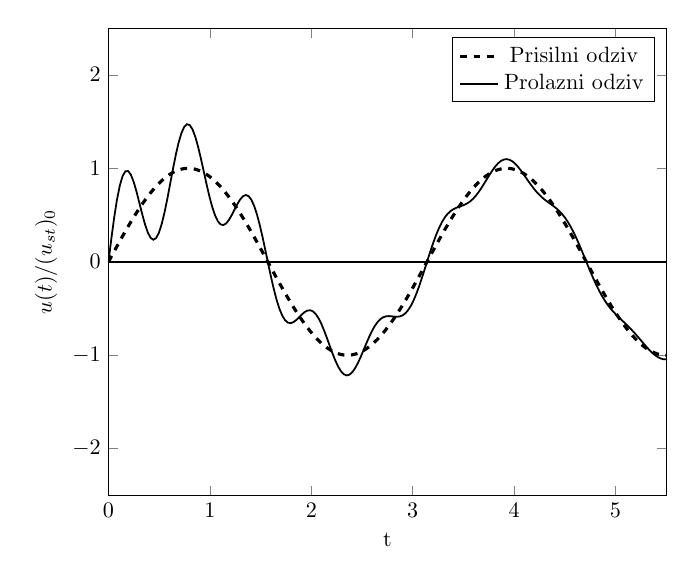
\begin{tikzpicture}[scale=0.8]
    \begin{axis} [
        height=9cm,
%        axis lines = center,
        xlabel=t,ylabel=$u(t)/(u_{st})_0$,
        ylabel near ticks, ylabel style={anchor=south},
        xmin = 0, xmax = 5.5,
        ymin = -2.5, ymax = 2.5,
        xtick = {0, 1, 2, 3, 4, 5},
        ytick = {-2,-1, 0, 1, 2},
     ]
        \addplot [
            domain=0:5.5,
            samples=200,
            color=black,
            dashed,line width=0.5mm,
        ] {sin(2*deg(x))};
        \addlegendentry{Prisilni odziv}
        \addplot [
            domain=0:5.5,
            samples=200,
            color=black,
            thick,
        ] {sin(2*deg(x))+0.7*exp(-0.05*10*x)*sin(10*deg(x))};
        \addlegendentry{Prolazni odziv}
    \draw[thick] (0,0)--(5.5,0);
    \end{axis}
\end{tikzpicture}
